% 必要な項目ができた場合は適宜サブセクションを追加してください

%\include{begin}

% イベント名を記入する
\section{起床}


% 日時と場所を記入する
% 時刻は4桁で記入すること!
\subsection{日時・場所}
\begin{tabular}{p{2zw}rp{38zw}}
  日時 & : & 2019年4月6日(土) 6:00 $\sim$ 7:10\\
  場所 & : & 幡多青少年の家本館
\end{tabular}


% イベントのタイムスケジュールを記入する
% 時刻は必ず4桁(00:00)で記入すること!
% 時間の流れは途切れないように記述する!
\subsection{タイムスケジュール}
\begin{longtable}{p{3zw}p{39zw}}
  06:00 & \textbf{◎ 新入生・先生方・スタッフ起床} \\
        & \ \ \textbullet \ \ 起床係は新入生,先生方を起こしに行く \\

        & \ \ \textbullet \ \ その他のスタッフは部屋の清掃,シーツ・布団の片付けを行う
        						(6:20までにできるだけ終わらせてスタッフ全員分の荷物の運搬をできるようにする) (図\ref{fig:futon_katazuke})\\
        & \ \ \textbullet \ \ 片付けが早く終わったスタッフは小松,西森,小島,三浦車にゴミを詰め込む \\
        & \ \ \textbullet \ \ 角原,渡辺,吉田,堀川は体調が悪い人がいないか,片付けの状態,その他気付いたことを報告slackに連絡する \\
        & \ \ \textbullet \ \ 体調が悪い人がいた場合,報告slackに報告後,妻鳥先生,幡多事務室と相談する \\
        & \ \ \textbullet \ \ 新入生を起こした後はシーツ・布団の片付けの指示を出す \\
        & \ \ \textbullet \ \ 部屋の掃除を分担して行うように指示を出す \\
        & \ \ \textbullet \ \ たたみ終わったシーツは各部屋でまとめて置くように指示する \\
        & \ \  ※朝食後に時間はあるが,なるべくこの時間で片付け・清掃などできることは終わるよう円滑に指示する \\
        & \ \ \textbullet \ \ 手の空いているスタッフは廊下,トイレ,各部屋を清掃する \\\\

  06:35 & \textbf{◎ 移動開始 } \\
\end{longtable}

% イベントに必要な役割と人数を記入する
% 担当者は決定次第追記する
% 記入例 ・司会者 2人(名前1、名前2)
\subsection{人員配置}
\begin{itemize}
\item 起床係(女子):角原,渡辺
\item 起床係(男子):吉田,堀川
\item 起床係(先生):小野,藤田(M2),以西,江川(女性教員)
%\item 宴のゴミの片付け:小島(車),野田,以西
\item ゴミを乗せる車:小島,小松,西森,三浦
\end{itemize}

\clearpage

% イベントに必要な物品と個数を記入する
% 記入例 ・マジックペン 10本
\subsection{布団のたたみ方}
\begin{figure}[h]
\begin{center}
\includegraphics[scale=0.5]{./16/futon_katazuke.eps}
\caption{布団のたたみ方}
\label{fig:futon_katazuke}
\end{center}
\end{figure}

\subsection{退所点検に向けて}
\begin{itemize}
\item シーツ・枕カバーをきれいにたたんでおく
\item 寝具・備品(ハンガー等)は元通りにする
\item 窓は閉めて,カーテンは開けて留めておく
\item 室内・廊下の掃除をし,ゴミ箱のゴミは研修生入り口のゴミ置き場に分別して処理する
\item 電気・エアコンの消し忘れをしない
\end{itemize}

% 注意事項やスタッフに周知しておくべきことがあれば記入する
\subsection{備考}
\begin{itemize}
\item 朝のつどいまでにベッド、部屋の片付けが完了しなければ朝食終了後に行う
\item スタッフはシーツのたたみ方を指導できるようにしておく
\item 体調不良者の対応を行う
\item 院生は先生を軽く起こして朝食の有無を聞く
\item 朝食がいらないと言われた場合,8:30には起床してもらうことを伝える
%\item 手の空いているスタッフは宴のゴミの片づけを手伝う
\item 起床係は6:35に正面広間に移動を開始することを新入生に伝える
\item 先生方が朝の集いに参加される場合は,小野,以西,藤田(M2)が誘導を行う

\end{itemize}

%\include{end}
